\documentclass{article}
\usepackage{iclr2026_conference,times}
\raggedbottom

%%%%% NEW MATH DEFINITIONS %%%%%

\usepackage{amsmath,amsfonts,bm}

% Mark sections of captions for referring to divisions of figures
\newcommand{\figleft}{{\em (Left)}}
\newcommand{\figcenter}{{\em (Center)}}
\newcommand{\figright}{{\em (Right)}}
\newcommand{\figtop}{{\em (Top)}}
\newcommand{\figbottom}{{\em (Bottom)}}
\newcommand{\captiona}{{\em (a)}}
\newcommand{\captionb}{{\em (b)}}
\newcommand{\captionc}{{\em (c)}}
\newcommand{\captiond}{{\em (d)}}

% Highlight a newly defined term
\newcommand{\newterm}[1]{{\bf #1}}


% Figure reference, lower-case.
\def\figref#1{figure~\ref{#1}}
% Figure reference, capital. For start of sentence
\def\Figref#1{Figure~\ref{#1}}
\def\twofigref#1#2{figures \ref{#1} and \ref{#2}}
\def\quadfigref#1#2#3#4{figures \ref{#1}, \ref{#2}, \ref{#3} and \ref{#4}}
% Section reference, lower-case.
\def\secref#1{section~\ref{#1}}
% Section reference, capital.
\def\Secref#1{Section~\ref{#1}}
% Reference to two sections.
\def\twosecrefs#1#2{sections \ref{#1} and \ref{#2}}
% Reference to three sections.
\def\secrefs#1#2#3{sections \ref{#1}, \ref{#2} and \ref{#3}}
% Reference to an equation, lower-case.
\def\eqref#1{equation~\ref{#1}}
% Reference to an equation, upper case
\def\Eqref#1{Equation~\ref{#1}}
% A raw reference to an equation---avoid using if possible
\def\plaineqref#1{\ref{#1}}
% Reference to a chapter, lower-case.
\def\chapref#1{chapter~\ref{#1}}
% Reference to an equation, upper case.
\def\Chapref#1{Chapter~\ref{#1}}
% Reference to a range of chapters
\def\rangechapref#1#2{chapters\ref{#1}--\ref{#2}}
% Reference to an algorithm, lower-case.
\def\algref#1{algorithm~\ref{#1}}
% Reference to an algorithm, upper case.
\def\Algref#1{Algorithm~\ref{#1}}
\def\twoalgref#1#2{algorithms \ref{#1} and \ref{#2}}
\def\Twoalgref#1#2{Algorithms \ref{#1} and \ref{#2}}
% Reference to a part, lower case
\def\partref#1{part~\ref{#1}}
% Reference to a part, upper case
\def\Partref#1{Part~\ref{#1}}
\def\twopartref#1#2{parts \ref{#1} and \ref{#2}}

\def\ceil#1{\lceil #1 \rceil}
\def\floor#1{\lfloor #1 \rfloor}
\def\1{\bm{1}}
\newcommand{\train}{\mathcal{D}}
\newcommand{\valid}{\mathcal{D_{\mathrm{valid}}}}
\newcommand{\test}{\mathcal{D_{\mathrm{test}}}}

\def\eps{{\epsilon}}


% Random variables
\def\reta{{\textnormal{$\eta$}}}
\def\ra{{\textnormal{a}}}
\def\rb{{\textnormal{b}}}
\def\rc{{\textnormal{c}}}
\def\rd{{\textnormal{d}}}
\def\re{{\textnormal{e}}}
\def\rf{{\textnormal{f}}}
\def\rg{{\textnormal{g}}}
\def\rh{{\textnormal{h}}}
\def\ri{{\textnormal{i}}}
\def\rj{{\textnormal{j}}}
\def\rk{{\textnormal{k}}}
\def\rl{{\textnormal{l}}}
% rm is already a command, just don't name any random variables m
\def\rn{{\textnormal{n}}}
\def\ro{{\textnormal{o}}}
\def\rp{{\textnormal{p}}}
\def\rq{{\textnormal{q}}}
\def\rr{{\textnormal{r}}}
\def\rs{{\textnormal{s}}}
\def\rt{{\textnormal{t}}}
\def\ru{{\textnormal{u}}}
\def\rv{{\textnormal{v}}}
\def\rw{{\textnormal{w}}}
\def\rx{{\textnormal{x}}}
\def\ry{{\textnormal{y}}}
\def\rz{{\textnormal{z}}}

% Random vectors
\def\rvepsilon{{\mathbf{\epsilon}}}
\def\rvtheta{{\mathbf{\theta}}}
\def\rva{{\mathbf{a}}}
\def\rvb{{\mathbf{b}}}
\def\rvc{{\mathbf{c}}}
\def\rvd{{\mathbf{d}}}
\def\rve{{\mathbf{e}}}
\def\rvf{{\mathbf{f}}}
\def\rvg{{\mathbf{g}}}
\def\rvh{{\mathbf{h}}}
\def\rvu{{\mathbf{i}}}
\def\rvj{{\mathbf{j}}}
\def\rvk{{\mathbf{k}}}
\def\rvl{{\mathbf{l}}}
\def\rvm{{\mathbf{m}}}
\def\rvn{{\mathbf{n}}}
\def\rvo{{\mathbf{o}}}
\def\rvp{{\mathbf{p}}}
\def\rvq{{\mathbf{q}}}
\def\rvr{{\mathbf{r}}}
\def\rvs{{\mathbf{s}}}
\def\rvt{{\mathbf{t}}}
\def\rvu{{\mathbf{u}}}
\def\rvv{{\mathbf{v}}}
\def\rvw{{\mathbf{w}}}
\def\rvx{{\mathbf{x}}}
\def\rvy{{\mathbf{y}}}
\def\rvz{{\mathbf{z}}}

% Elements of random vectors
\def\erva{{\textnormal{a}}}
\def\ervb{{\textnormal{b}}}
\def\ervc{{\textnormal{c}}}
\def\ervd{{\textnormal{d}}}
\def\erve{{\textnormal{e}}}
\def\ervf{{\textnormal{f}}}
\def\ervg{{\textnormal{g}}}
\def\ervh{{\textnormal{h}}}
\def\ervi{{\textnormal{i}}}
\def\ervj{{\textnormal{j}}}
\def\ervk{{\textnormal{k}}}
\def\ervl{{\textnormal{l}}}
\def\ervm{{\textnormal{m}}}
\def\ervn{{\textnormal{n}}}
\def\ervo{{\textnormal{o}}}
\def\ervp{{\textnormal{p}}}
\def\ervq{{\textnormal{q}}}
\def\ervr{{\textnormal{r}}}
\def\ervs{{\textnormal{s}}}
\def\ervt{{\textnormal{t}}}
\def\ervu{{\textnormal{u}}}
\def\ervv{{\textnormal{v}}}
\def\ervw{{\textnormal{w}}}
\def\ervx{{\textnormal{x}}}
\def\ervy{{\textnormal{y}}}
\def\ervz{{\textnormal{z}}}

% Random matrices
\def\rmA{{\mathbf{A}}}
\def\rmB{{\mathbf{B}}}
\def\rmC{{\mathbf{C}}}
\def\rmD{{\mathbf{D}}}
\def\rmE{{\mathbf{E}}}
\def\rmF{{\mathbf{F}}}
\def\rmG{{\mathbf{G}}}
\def\rmH{{\mathbf{H}}}
\def\rmI{{\mathbf{I}}}
\def\rmJ{{\mathbf{J}}}
\def\rmK{{\mathbf{K}}}
\def\rmL{{\mathbf{L}}}
\def\rmM{{\mathbf{M}}}
\def\rmN{{\mathbf{N}}}
\def\rmO{{\mathbf{O}}}
\def\rmP{{\mathbf{P}}}
\def\rmQ{{\mathbf{Q}}}
\def\rmR{{\mathbf{R}}}
\def\rmS{{\mathbf{S}}}
\def\rmT{{\mathbf{T}}}
\def\rmU{{\mathbf{U}}}
\def\rmV{{\mathbf{V}}}
\def\rmW{{\mathbf{W}}}
\def\rmX{{\mathbf{X}}}
\def\rmY{{\mathbf{Y}}}
\def\rmZ{{\mathbf{Z}}}

% Elements of random matrices
\def\ermA{{\textnormal{A}}}
\def\ermB{{\textnormal{B}}}
\def\ermC{{\textnormal{C}}}
\def\ermD{{\textnormal{D}}}
\def\ermE{{\textnormal{E}}}
\def\ermF{{\textnormal{F}}}
\def\ermG{{\textnormal{G}}}
\def\ermH{{\textnormal{H}}}
\def\ermI{{\textnormal{I}}}
\def\ermJ{{\textnormal{J}}}
\def\ermK{{\textnormal{K}}}
\def\ermL{{\textnormal{L}}}
\def\ermM{{\textnormal{M}}}
\def\ermN{{\textnormal{N}}}
\def\ermO{{\textnormal{O}}}
\def\ermP{{\textnormal{P}}}
\def\ermQ{{\textnormal{Q}}}
\def\ermR{{\textnormal{R}}}
\def\ermS{{\textnormal{S}}}
\def\ermT{{\textnormal{T}}}
\def\ermU{{\textnormal{U}}}
\def\ermV{{\textnormal{V}}}
\def\ermW{{\textnormal{W}}}
\def\ermX{{\textnormal{X}}}
\def\ermY{{\textnormal{Y}}}
\def\ermZ{{\textnormal{Z}}}

% Vectors
\def\vzero{{\bm{0}}}
\def\vone{{\bm{1}}}
\def\vmu{{\bm{\mu}}}
\def\vtheta{{\bm{\theta}}}
\def\va{{\bm{a}}}
\def\vb{{\bm{b}}}
\def\vc{{\bm{c}}}
\def\vd{{\bm{d}}}
\def\ve{{\bm{e}}}
\def\vf{{\bm{f}}}
\def\vg{{\bm{g}}}
\def\vh{{\bm{h}}}
\def\vi{{\bm{i}}}
\def\vj{{\bm{j}}}
\def\vk{{\bm{k}}}
\def\vl{{\bm{l}}}
\def\vm{{\bm{m}}}
\def\vn{{\bm{n}}}
\def\vo{{\bm{o}}}
\def\vp{{\bm{p}}}
\def\vq{{\bm{q}}}
\def\vr{{\bm{r}}}
\def\vs{{\bm{s}}}
\def\vt{{\bm{t}}}
\def\vu{{\bm{u}}}
\def\vv{{\bm{v}}}
\def\vw{{\bm{w}}}
\def\vx{{\bm{x}}}
\def\vy{{\bm{y}}}
\def\vz{{\bm{z}}}

% Elements of vectors
\def\evalpha{{\alpha}}
\def\evbeta{{\beta}}
\def\evepsilon{{\epsilon}}
\def\evlambda{{\lambda}}
\def\evomega{{\omega}}
\def\evmu{{\mu}}
\def\evpsi{{\psi}}
\def\evsigma{{\sigma}}
\def\evtheta{{\theta}}
\def\eva{{a}}
\def\evb{{b}}
\def\evc{{c}}
\def\evd{{d}}
\def\eve{{e}}
\def\evf{{f}}
\def\evg{{g}}
\def\evh{{h}}
\def\evi{{i}}
\def\evj{{j}}
\def\evk{{k}}
\def\evl{{l}}
\def\evm{{m}}
\def\evn{{n}}
\def\evo{{o}}
\def\evp{{p}}
\def\evq{{q}}
\def\evr{{r}}
\def\evs{{s}}
\def\evt{{t}}
\def\evu{{u}}
\def\evv{{v}}
\def\evw{{w}}
\def\evx{{x}}
\def\evy{{y}}
\def\evz{{z}}

% Matrix
\def\mA{{\bm{A}}}
\def\mB{{\bm{B}}}
\def\mC{{\bm{C}}}
\def\mD{{\bm{D}}}
\def\mE{{\bm{E}}}
\def\mF{{\bm{F}}}
\def\mG{{\bm{G}}}
\def\mH{{\bm{H}}}
\def\mI{{\bm{I}}}
\def\mJ{{\bm{J}}}
\def\mK{{\bm{K}}}
\def\mL{{\bm{L}}}
\def\mM{{\bm{M}}}
\def\mN{{\bm{N}}}
\def\mO{{\bm{O}}}
\def\mP{{\bm{P}}}
\def\mQ{{\bm{Q}}}
\def\mR{{\bm{R}}}
\def\mS{{\bm{S}}}
\def\mT{{\bm{T}}}
\def\mU{{\bm{U}}}
\def\mV{{\bm{V}}}
\def\mW{{\bm{W}}}
\def\mX{{\bm{X}}}
\def\mY{{\bm{Y}}}
\def\mZ{{\bm{Z}}}
\def\mBeta{{\bm{\beta}}}
\def\mPhi{{\bm{\Phi}}}
\def\mLambda{{\bm{\Lambda}}}
\def\mSigma{{\bm{\Sigma}}}

% Tensor
\DeclareMathAlphabet{\mathsfit}{\encodingdefault}{\sfdefault}{m}{sl}
\SetMathAlphabet{\mathsfit}{bold}{\encodingdefault}{\sfdefault}{bx}{n}
\newcommand{\tens}[1]{\bm{\mathsfit{#1}}}
\def\tA{{\tens{A}}}
\def\tB{{\tens{B}}}
\def\tC{{\tens{C}}}
\def\tD{{\tens{D}}}
\def\tE{{\tens{E}}}
\def\tF{{\tens{F}}}
\def\tG{{\tens{G}}}
\def\tH{{\tens{H}}}
\def\tI{{\tens{I}}}
\def\tJ{{\tens{J}}}
\def\tK{{\tens{K}}}
\def\tL{{\tens{L}}}
\def\tM{{\tens{M}}}
\def\tN{{\tens{N}}}
\def\tO{{\tens{O}}}
\def\tP{{\tens{P}}}
\def\tQ{{\tens{Q}}}
\def\tR{{\tens{R}}}
\def\tS{{\tens{S}}}
\def\tT{{\tens{T}}}
\def\tU{{\tens{U}}}
\def\tV{{\tens{V}}}
\def\tW{{\tens{W}}}
\def\tX{{\tens{X}}}
\def\tY{{\tens{Y}}}
\def\tZ{{\tens{Z}}}


% Graph
\def\gA{{\mathcal{A}}}
\def\gB{{\mathcal{B}}}
\def\gC{{\mathcal{C}}}
\def\gD{{\mathcal{D}}}
\def\gE{{\mathcal{E}}}
\def\gF{{\mathcal{F}}}
\def\gG{{\mathcal{G}}}
\def\gH{{\mathcal{H}}}
\def\gI{{\mathcal{I}}}
\def\gJ{{\mathcal{J}}}
\def\gK{{\mathcal{K}}}
\def\gL{{\mathcal{L}}}
\def\gM{{\mathcal{M}}}
\def\gN{{\mathcal{N}}}
\def\gO{{\mathcal{O}}}
\def\gP{{\mathcal{P}}}
\def\gQ{{\mathcal{Q}}}
\def\gR{{\mathcal{R}}}
\def\gS{{\mathcal{S}}}
\def\gT{{\mathcal{T}}}
\def\gU{{\mathcal{U}}}
\def\gV{{\mathcal{V}}}
\def\gW{{\mathcal{W}}}
\def\gX{{\mathcal{X}}}
\def\gY{{\mathcal{Y}}}
\def\gZ{{\mathcal{Z}}}

% Sets
\def\sA{{\mathbb{A}}}
\def\sB{{\mathbb{B}}}
\def\sC{{\mathbb{C}}}
\def\sD{{\mathbb{D}}}
% Don't use a set called E, because this would be the same as our symbol
% for expectation.
\def\sF{{\mathbb{F}}}
\def\sG{{\mathbb{G}}}
\def\sH{{\mathbb{H}}}
\def\sI{{\mathbb{I}}}
\def\sJ{{\mathbb{J}}}
\def\sK{{\mathbb{K}}}
\def\sL{{\mathbb{L}}}
\def\sM{{\mathbb{M}}}
\def\sN{{\mathbb{N}}}
\def\sO{{\mathbb{O}}}
\def\sP{{\mathbb{P}}}
\def\sQ{{\mathbb{Q}}}
\def\sR{{\mathbb{R}}}
\def\sS{{\mathbb{S}}}
\def\sT{{\mathbb{T}}}
\def\sU{{\mathbb{U}}}
\def\sV{{\mathbb{V}}}
\def\sW{{\mathbb{W}}}
\def\sX{{\mathbb{X}}}
\def\sY{{\mathbb{Y}}}
\def\sZ{{\mathbb{Z}}}

% Entries of a matrix
\def\emLambda{{\Lambda}}
\def\emA{{A}}
\def\emB{{B}}
\def\emC{{C}}
\def\emD{{D}}
\def\emE{{E}}
\def\emF{{F}}
\def\emG{{G}}
\def\emH{{H}}
\def\emI{{I}}
\def\emJ{{J}}
\def\emK{{K}}
\def\emL{{L}}
\def\emM{{M}}
\def\emN{{N}}
\def\emO{{O}}
\def\emP{{P}}
\def\emQ{{Q}}
\def\emR{{R}}
\def\emS{{S}}
\def\emT{{T}}
\def\emU{{U}}
\def\emV{{V}}
\def\emW{{W}}
\def\emX{{X}}
\def\emY{{Y}}
\def\emZ{{Z}}
\def\emSigma{{\Sigma}}

% entries of a tensor
% Same font as tensor, without \bm wrapper
\newcommand{\etens}[1]{\mathsfit{#1}}
\def\etLambda{{\etens{\Lambda}}}
\def\etA{{\etens{A}}}
\def\etB{{\etens{B}}}
\def\etC{{\etens{C}}}
\def\etD{{\etens{D}}}
\def\etE{{\etens{E}}}
\def\etF{{\etens{F}}}
\def\etG{{\etens{G}}}
\def\etH{{\etens{H}}}
\def\etI{{\etens{I}}}
\def\etJ{{\etens{J}}}
\def\etK{{\etens{K}}}
\def\etL{{\etens{L}}}
\def\etM{{\etens{M}}}
\def\etN{{\etens{N}}}
\def\etO{{\etens{O}}}
\def\etP{{\etens{P}}}
\def\etQ{{\etens{Q}}}
\def\etR{{\etens{R}}}
\def\etS{{\etens{S}}}
\def\etT{{\etens{T}}}
\def\etU{{\etens{U}}}
\def\etV{{\etens{V}}}
\def\etW{{\etens{W}}}
\def\etX{{\etens{X}}}
\def\etY{{\etens{Y}}}
\def\etZ{{\etens{Z}}}

% The true underlying data generating distribution
\newcommand{\pdata}{p_{\rm{data}}}
% The empirical distribution defined by the training set
\newcommand{\ptrain}{\hat{p}_{\rm{data}}}
\newcommand{\Ptrain}{\hat{P}_{\rm{data}}}
% The model distribution
\newcommand{\pmodel}{p_{\rm{model}}}
\newcommand{\Pmodel}{P_{\rm{model}}}
\newcommand{\ptildemodel}{\tilde{p}_{\rm{model}}}
% Stochastic autoencoder distributions
\newcommand{\pencode}{p_{\rm{encoder}}}
\newcommand{\pdecode}{p_{\rm{decoder}}}
\newcommand{\precons}{p_{\rm{reconstruct}}}

\newcommand{\laplace}{\mathrm{Laplace}} % Laplace distribution

\newcommand{\E}{\mathbb{E}}
\newcommand{\Ls}{\mathcal{L}}
\newcommand{\R}{\mathbb{R}}
\newcommand{\emp}{\tilde{p}}
\newcommand{\lr}{\alpha}
\newcommand{\reg}{\lambda}
\newcommand{\rect}{\mathrm{rectifier}}
\newcommand{\softmax}{\mathrm{softmax}}
\newcommand{\sigmoid}{\sigma}
\newcommand{\softplus}{\zeta}
\newcommand{\KL}{D_{\mathrm{KL}}}
\newcommand{\Var}{\mathrm{Var}}
\newcommand{\standarderror}{\mathrm{SE}}
\newcommand{\Cov}{\mathrm{Cov}}
% Wolfram Mathworld says $L^2$ is for function spaces and $\ell^2$ is for vectors
% But then they seem to use $L^2$ for vectors throughout the site, and so does
% wikipedia.
\newcommand{\normlzero}{L^0}
\newcommand{\normlone}{L^1}
\newcommand{\normltwo}{L^2}
\newcommand{\normlp}{L^p}
\newcommand{\normmax}{L^\infty}

\newcommand{\parents}{Pa} % See usage in notation.tex. Chosen to match Daphne's book.

\DeclareMathOperator*{\argmax}{arg\,max}
\DeclareMathOperator*{\argmin}{arg\,min}

\DeclareMathOperator{\sign}{sign}
\DeclareMathOperator{\Tr}{Tr}
\let\ab\allowbreak


\usepackage{hyperref}
\usepackage{url}
\usepackage{graphicx}
\usepackage{booktabs}
\usepackage{tabularx}
\usepackage{array}
\usepackage{xcolor}

\title{Full Fine-Tuning Versus Parameter-Efficient Adaptation of a Vision
Transformer for 10,000-Class Fine-Grained Classification}

\author{Anastasia Frances Frederica, Le Thi Hong Van, Liu Wenqi \& Xu Qianqian \\
CS604 Team 08 \\
Singapore Management University}

\iclrfinalcopy

% \iclrfinalcopy keeps the author names. The style then writes
% "Published as a conference paper at ICLR 2026" from inside \maketitle,
% and a later \pagestyle{fancy} would put that line back. Install the
% course header whenever the fancy page style is applied.
\makeatletter
\let\course@origfancy\ps@@fancy
\def\ps@@fancy{%
  \course@origfancy
  \def\@oddhead{\hfill CS604 Course Project Report\hfill}%
  \def\@evenhead{\hfill CS604 Course Project Report\hfill}%
}
\pagestyle{fancy}
\let\course@origtitle\maketitle
\def\maketitle{\course@origtitle\fancyhead{}\pagestyle{fancy}}
\makeatother

% Keep figures and tables in source order. A normal float can jump
% above its section or into the reference list.
\newcommand{\stayfig}[3]{%
  \par\vspace{0.35em}%
  \noindent\begin{minipage}{\textwidth}%
  \centering
  #1\par\vspace{0.2em}%
  \refstepcounter{figure}\label{#3}%
  {\small Figure~\thefigure: #2\par}%
  \end{minipage}%
  \par\vspace{0.15em}%
}
\newcommand{\staytable}[3]{%
  \par\vspace{0.45em}%
  \noindent\begin{minipage}{\textwidth}%
  \centering
  \refstepcounter{table}\label{#3}%
  {\small Table~\thetable: #2\par}%
  \vspace{0.2em}%
  #1%
  \end{minipage}%
  \par\vspace{0.2em}%
}
\setlength{\bibsep}{1.5pt plus 0.5pt minus 0.5pt}

\begin{document}
\maketitle
\begin{abstract}
Pretrained Vision Transformers can be adapted to a new task by fine-tuning every weight or parameter-efficient fine-tuning (PEFT). We compare the two on 10,000 fine-grained classes with 45 training images each, and a fixed per-run compute budget (Section 3.1). We ask how close PEFT gets to a well-tuned full fine-tune, how a fixed PEFT budget should be spent, and what limits the adapted model. On the validation set, full fine-tuning with a prototype-initialised cosine head, layer-wise learning-rate decay and 448 px training achieves 84.07\% top-1 accuracy. AdaptFormer with LoRA, training 4.94\% of the backbone, achieves 83.08\%: within 1.0 percentage point, with less memory but no reduction in training time and slower inference. The choice of trainable parameters matters more than their quantity. Most remaining errors are near misses: the true class is in the top five for 64\% of them. An attention-guided zoom and kNN re-ranking against individual training images add 1.6--2.0 pp without retraining, and the best model reaches 83.84\% on the unseen test set, only 0.23 pp below its validation score. Adapting a pretrained model is a joint design problem: resolution, optimisation, parameter allocation and prediction all interact.
\end{abstract}

\section{Introduction}\label{introduction}

Vision Transformers (ViTs) match or outperform convolutional networks given enough pretraining data, but because they lack built-in inductive biases such as locality, training one from scratch is expensive and data-hungry \citep{dosovitskiy2021vit}. In practice, a pretrained ViT is therefore adapted to the downstream task through transfer learning. Full fine-tuning updates every weight. This is the most flexible option, but it needs the most memory and can distort useful pretrained features \citep{kumar2022lpft}. Parameter-efficient fine-tuning (PEFT) instead trains a small set of parameters, which saves memory but may cost accuracy or add inference latency. Choosing between them therefore takes more than comparing trainable-parameter counts, because training time, GPU memory and latency all constrain deployment.

We compare the two on a 10,000-class fine-grained task with only 45 training images per class. Classes look alike, and images within a class vary widely. Pretrained features alone reach only 43.9\% with a nearest-class-centroid classifier. All runs start from the same ViT-B/16 checkpoint (86M parameters) under a fixed per-run compute budget (Section 3.1). We ask three research questions:

\begin{itemize}
\item
  \textbf{RQ1. Full fine-tuning versus PEFT:} Under the same computational budget, how do full fine-tuning and PEFT (under 5\% trainable parameters) compare in accuracy, training efficiency, memory consumption and inference latency?
\item
  \textbf{RQ2. Allocation of PEFT capacity:} How does the adaptation method, parameter placement and type of added capacity influence accuracy within a fixed parameter budget?
\item
  \textbf{RQ3. Residual classification errors:} What errors persist after adaptation, and can training-free prediction-time techniques reduce them?
\end{itemize}

\section{Related work}\label{related-work}

\textbf{Pretrained Vision Transformers.} AugReg \citep{steiner2022augreg} showed that strong augmentation and regularisation partly substitute for pretraining data; we start from its ViT-B/16 checkpoint (pretrained on ImageNet-21k, fine-tuned on ImageNet-1k). When full fine-tuning starts from a random head, early updates can distort the pretrained features; LP-FT avoids this by training a linear probe first \citep{kumar2022lpft}. Weight imprinting instead initialises each class weight to the mean feature of that class \citep{qi2018imprinting}, which pairs naturally with a cosine classifier; CosFace adds a margin to make the features more discriminative \citep{wang2018cosface}. Layer-wise learning-rate decay gives earlier, more general layers smaller updates and is standard in ViT fine-tuning recipes \citep{he2022mae}. We adopt the cosine classifier and layer-wise decay, and compare prototype initialisation against LP-FT.

\textbf{Parameter-efficient fine-tuning.} PEFT methods differ in what they train, and therefore in what they cost. Selective methods tune existing weights, such as the biases (BitFit; \citealp{zaken2022bitfit}), gradient-selected parameters (GPS; \citealp{zhang2024gps}) or chosen layers \citep{lee2023surgical}. They add no inference cost but have limited capacity. Additive methods insert new modules: prompt tokens \citep{li2021prefix,jia2022vpt}, serial bottleneck adapters \citep{houlsby2019adapter} or a parallel MLP branch (AdaptFormer; \citealp{chen2022adaptformer}). They are flexible but stay in the forward pass, so they add latency. Reparameterisation methods such as LoRA \citep{hu2022lora}, DoRA \citep{liu2024dora} and AdaLoRA \citep{zhang2023adalora} learn low-rank weight updates that can be merged after training, so they add no inference cost, but the rank caps their capacity. Section 5.3 measures these trade-offs under one budget.

\textbf{Prediction-time methods.} RA-CNN \citep{fu2017racnn} zooms into the region its attention finds most discriminative, but it trains extra attention modules. Our zoom takes the region from the trained model's own patch-to-class similarity, so it trains nothing. Nearest-neighbour classifiers compare a query with stored training features \citep{wu2018instance}. Unlike class means \citep{mensink2013ncm}, they keep a class's rare appearances. Like kNN-LM \citep{khandelwal2020knnlm}, we add neighbour similarity to the model's own score.

\textbf{Positioning.} PEFT methods are usually compared by accuracy at a given number of trainable parameters \citep[e.g.,][]{hu2022lora,jia2022vpt,chen2022adaptformer}. We instead compare full fine-tuning and PEFT at an equal wall-clock budget, report memory, training time and latency separately, and treat the head's initialisation, the input resolution and the prediction step as part of the adaptation method.

\section{Method}\label{method}

\subsection{Dataset, Setup and Budget}\label{dataset-setup-and-budget}

\textbf{Dataset.} We use the CS604 course project dataset \citep{cs604data}, an anonymised fine-grained image classification dataset with 10,000 classes. It provides 450,000 labelled training images (45 per class), a validation set of 50,000 images (5 per class) and a test set of 100,000 images (10 per class). Validation and test labels are not available to us, so both sets are scored only on the evaluation server (Section 4). Class names are anonymised, so no class semantics or hierarchy is available.

\textbf{Model.} We adapt a ViT-B/16 backbone (timm vit\_base\_patch16\_224.augreg2\_in21k\_ft\_in1k; \citealp{rw2019timm}; 86M parameters) to these 10,000 classes. The classification head is always trained and is not counted towards the 5\% PEFT budget, which applies only to the backbone.

\textbf{Budget}. The project budget for each run is 96 GB-hours, equivalent to 2 hours on a 48 GB GPU. On the 40 GB A100 we used, this corresponds to 144 minutes (2.4 GPU-hours) per run. Every model evaluated on the validation and test sets was trained for exactly this budget, with training stopped when the time ran out. Fixing the wall-clock budget, rather than the number of epochs, lets us compare full fine-tuning and PEFT under the same practical constraint. The shorter holdout and pilot runs used for development are described in Section 4. Three steps that train no parameters run outside the 144-minute limit: computing the class prototypes that initialise the head (one frozen pass over all 450,000 training images at 448 px, about 18 min), the PCA initialisation of AdaptFormer (about 10 s), and building the kNN feature bank (about 25--30 min).

\subsection{Overview}\label{overview}

We train two routes, full fine-tuning and PEFT, that differ only in how the backbone is adapted (Figure~\ref{fig:pipeline}): both use the same pretrained ViT, prototype cosine head, 448 px input and prediction steps, and each route\textquotesingle s training recipe is tuned separately (Sections 3.3 and 3.5). Our changes fall into four groups: how the head starts, how fast each block learns, how much detail the model sees, and how predictions are made.

\stayfig{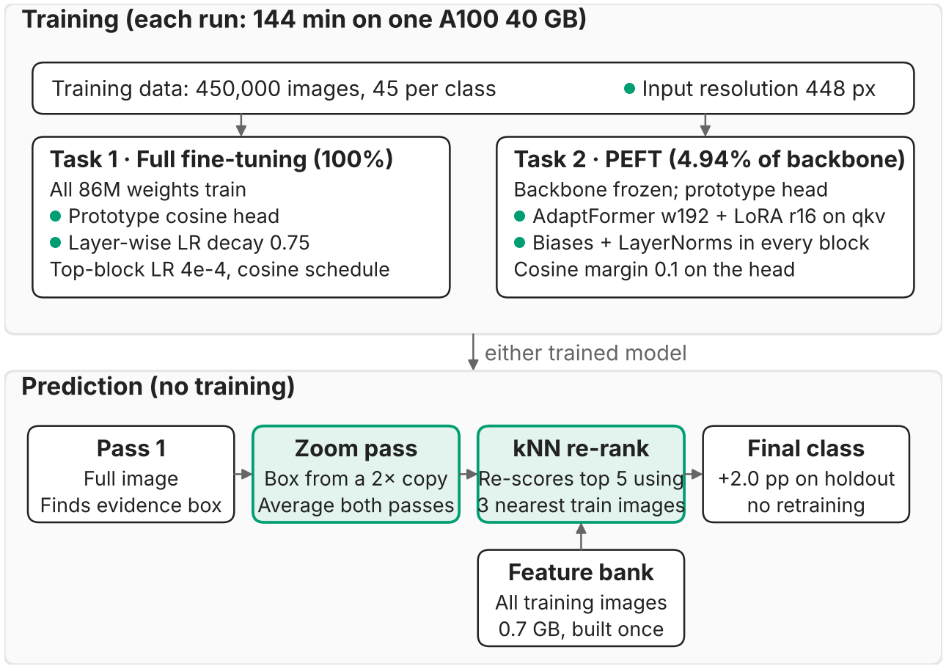
\includegraphics[width=0.72\textwidth]{media/media/image1.png}}{Pipeline for the full fine-tuning and PEFT routes. Dots mark our changes; shaded boxes are prediction-time steps.}{fig:pipeline}


\subsection{A full fine-tuning recipe that keeps the pretrained features}\label{a-full-fine-tuning-recipe-that-keeps-the-pretrained-features}

Our initial full fine-tune, with a single small learning rate for all blocks and no schedule, reached 61.3\% on the validation set, below a linear probe on frozen features (62.5\%), which is consistent with the feature distortion described by \citet{kumar2022lpft}. A fair comparison with PEFT (RQ1) requires a full fine-tuning baseline that avoids this, so we made four changes.

\begin{itemize}
\item
  \textbf{Prototype cosine head.} Each class weight starts at the normalised mean pretrained feature of that class\textquotesingle s training images. Logits are cosine similarities times a learned temperature. Why not LP-FT: a trained linear probe already attains low training loss, so it backpropagates only small gradients to the backbone. Prototypes give a reasonable but uncalibrated starting point with higher initial loss, so the backbone continues to adapt (+1.6 pp over LP-FT; Section 5.2).
\item
  \textbf{Layer-wise learning-rate decay.} The final norm learns at 4e-4 and each block below at 0.75$\times$ the rate of the one above, following \citet{he2022mae}; the top rate came from a five-point sweep (Appendix, Figure~\ref{fig:lr-sweep}). This lets the top blocks adapt quickly while limiting changes to the early blocks; removing it costs 6.71 pp on the holdout (Table~\ref{tab:ft-ablation}).
\item
  \textbf{Head learning rate 10$\times$ the backbone (4e-3).} The head is new and must move faster than a backbone that only needs nudging (+1.5 pp, Section 5.2).
\item
  \textbf{Time-based schedule.} After a 5\% warm-up, the learning rate follows a cosine decay driven by elapsed wall-clock time rather than step count, so it reaches zero exactly at the 144-minute limit. Holding the peak rate after warm-up instead of decaying it lowered holdout accuracy by 9.0 pp at 3 epochs (63.99\% vs. 72.98\%; Table~\ref{tab:ft-ablation}).
\end{itemize}

Untuned settings follow the MAE ViT-B fine-tuning recipe \citep{he2022mae}: label smoothing 0.1, drop path 0.1, AdamW weight decay 0.05 (none on norms and biases), and gradient clipping at norm 1.0 as in the original ViT fine-tuning \citep{dosovitskiy2021vit}. Each weight update uses 256 images; the 448 px finals process them as four accumulated batches of 64 (no gradient checkpointing), in bf16. Together, these changes raise full fine-tuning at 224 px to 75.7\% on the validation set (Section 5.2).

\subsection{Trade-off between epochs and resolution}\label{trade-off-between-epochs-and-resolution}

With 16$\times$16 patches, a small object spanning 12 patches at 224 px spans about 48 at 448 px, and most images (79\%) have a short side of 300--400 px, so training at 224 px discards detail. Four times as many patches make each step slower, so under a fixed budget resolution trades off against epochs. We train at 448 px because at equal compute it beat both extra epochs and low-to-high resolution schedules (Section 5.2).

\subsection{PEFT design: AdaptFormer + LoRA under 5\%}\label{peft-design-adaptformer-lora-under-5}

We freeze the backbone and add three sets of trainable parameters, 4,262,412 in total (4.94\% of the 86,250,240-parameter backbone):

\begin{itemize}
\item
  \textbf{AdaptFormer} (3,550,476 parameters). Each transformer block gets a lightweight bottleneck branch that runs in parallel with its MLP. The branch projects features down from 768 to 192 dimensions, applies a ReLU, projects back up to 768, and multiplies the output by a learned per-block scale. The up-projection is initialised to zero, so at the start of training the model's outputs are identical to those of the pretrained model. The down-projection is initialised from a principal component analysis (PCA) of the backbone features.
\item
  \textbf{Bias and LayerNorm tuning} (122,112 parameters; 0.14\% of the backbone). The existing bias terms and LayerNorm weights in every block are unfrozen.
\item
  \textbf{LoRA} (589,824 parameters). A rank-16 low-rank update is added to the query--key--value (qkv) projection in each block.
\end{itemize}

The percentage counts all trainable backbone-side parameters (added modules plus unfrozen biases and LayerNorm weights) relative to the backbone at 448 px; the 10,000-class head (7.68M parameters) is counted separately. A new task needs only about 17 MB of adapter weights and a 31 MB head, against 375 MB for a full fine-tune.

\textbf{Training configuration.} We follow Section 3.3 (including the head learning rate of 4e-3) with two changes: all trainable backbone-side parameters share one learning rate of 1e-3 without layer-wise decay, and a CosFace margin of 0.1 is applied to the cosine head. The margin was tuned with AdaptFormer only; in a LoRA-only pilot its effect was negligible (+0.18 pp).

\textbf{Design rationale.} Components were added one at a time and kept only if they improved holdout accuracy (Section 5.3). LoRA alone matched AdaptFormer + LoRA at the same budget; we kept AdaptFormer because it trains about 20\% faster, at the cost of slower inference, since its non-linear branch cannot be merged into the weights.

\subsection{Prediction-time extensions (no training)}\label{prediction-time-extensions-no-training}

\textbf{Zoom.} Higher input resolution helped during training (Section 5.2), so zoom applies the same idea at prediction time. After the first forward pass, we build a class activation map \citep{zhou2016cam} from the cosine similarity between each patch token and the predicted class's head weight. We find the smallest window containing 70\% of the total activation, crop it from a 2$\times$ upsampled copy of the image, and classify the crop with the same model. The prediction averages the softmax outputs of the full image and the crop.

\textbf{kNN re-ranking.} In 64\% of errors the true class is still in the top five (Section 5.5), so we re-score the top K candidates by how closely the query matches individual training images of each class:

\begin{equation}
s(c)=\log p(c\mid x)+\beta\frac{1}{m}\sum_{i\in\mathrm{top}\text{-}m}
\cos\!\left(f(x),f(x_i^c)\right).
\end{equation}
Here $f$ is the trained model's feature extractor, and the sum runs over the m training images of class c most similar to the query. The feature bank covers all 450,000 training images (0.7 GB in fp16) and is computed once. We set K = 5, m = 3 and $\beta$ = 20 by two-fold cross-validation over holdout classes (both folds agreed).

\section{Experimental setup}\label{experimental-setup}

\textbf{Evaluation protocol.} We screen ideas on a 1,000-class pilot, tune and run controlled comparisons on a labelled holdout (5 training images per class held out from all 10,000 classes), compare final systems on the validation set, and use the test set once, to check the best model for overfitting. The server allows only a few submissions, so we test each design change on the holdout, where we can run as many comparisons as needed. Pilot results are compared only with each other, because ten times fewer classes inflate their accuracy. We treat holdout differences below 0.4 pp as ties: a second seed on six configurations changed accuracy by at most 0.14 pp, and the largest spread we observed was 0.33 pp.

\textbf{Metrics.} We report top-1 accuracy, the trainable parameter share relative to the backbone, peak training memory, the number of training epochs completed within the fixed budget and inference latency. Latency is measured on a single A100 in bf16 as the forward-pass time on inputs already on the GPU, using 30 warm-up and 200 timed iterations, and excludes image loading and preprocessing. Batch-1 latency varies by about 1 ms between sessions, so the two final systems were timed in the same session.

\section{Results and analysis}\label{results-and-analysis}

\subsection{Main results}\label{main-results}

Full fine-tuning beats PEFT both without extensions (82.5\% vs 81.2\%) and with zoom and kNN (84.07\% vs 83.08\%; Table~\ref{tab:final}). On the unseen test set, the final full fine-tuning system reaches 83.84\%, 0.23 pp below its validation score (Section 5.4). PEFT was not scored on the test set, because only two test submissions were allowed, so the comparison between the two methods uses the validation set. PEFT trains 4.94\% of the backbone and uses 3.1 GiB less peak memory at the same physical batch, but it does not reduce training time: both methods complete 5.5 epochs in 144 minutes. PEFT is also slower at inference (11.27 vs 8.47 ms per image; 13.45 ms before LoRA is merged), though this comes from our choice of AdaptFormer rather than from PEFT as such (summary of all measures in Appendix, Figure~\ref{fig:summary}).



\staytable{%
\small
\begin{tabularx}{\textwidth}{@{}Xcc@{}}
\toprule
Metric & Full FT & AF + LoRA (PEFT) \\
\midrule
Validation top-1 (\%), no extensions / +zoom / +zoom+kNN & 82.5 / 83.22 / 84.07 & 81.2 / 82.2 / 83.08 \\
Trainable share of backbone & 100\% & 4.94\% \\
Peak training VRAM (GiB) & 17.80 & 14.66 \\
Epochs in 144 min & 5.5 & 5.5 \\
Latency, one pass (ms) & 8.47 & 11.27 (13.45 unmerged) \\
Latency with zoom (ms) & 23.43 & 29.88 \\
\bottomrule
\end{tabularx}}{Comparison of the final systems on the validation set (448 px, 144 training minutes on one A100). Latency is batch 1; peak VRAM uses physical batch 64.}{tab:final}


Both final runs were still improving when the 144-minute limit ended training: their epoch-mean loss fell in every epoch (Figure~\ref{fig:loss}). More time would likely have helped both, but Section 5.2 shows that, at equal compute, higher resolution gains more than extra epochs.

\stayfig{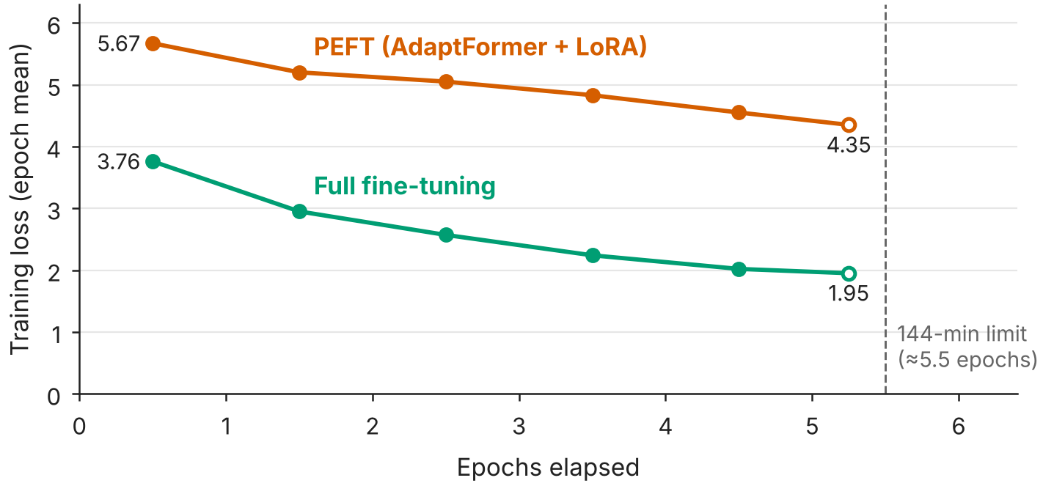
\includegraphics[width=0.68\textwidth]{media/media/image2.png}}{Epoch-mean training loss of the final systems at 448 px. The dashed line marks the 144-minute limit (about 5.5 epochs).}{fig:loss}


\subsection{Full fine-tuning ablations}\label{full-fine-tuning-ablations}

Most of the improvement over the initial baseline comes from two sources: the training recipe and the input resolution. Starting from the initial 61.3\% at 224 px, a prototype-initialised head (62.1\%) and a learning-rate schedule decaying to zero (66.3\%) gave the first gains; the remaining changes of Section 3.3 then raise validation accuracy to 75.7\%. Raising the input resolution then lifts it to 80.7\% at 336 px, 81.7\% at 384 px and 82.5\% at 448 px (+6.8 pp in total). These runs were not fully controlled, so the per-step gains are approximate. Zoom and kNN add a further 0.72 and 0.85 pp, reaching 84.07\%.



\staytable{%
\small
\begin{tabularx}{\textwidth}{@{}Xccc@{}}
\toprule
Setting & Top-1 (\%) & Change & Compared with \\
\midrule
Pretrained features, prototype head, no training & 43.90 & -- & -- \\
Control: LP-FT head at backbone LR & 69.83 & -- & -- \\
+ head LR $10\times$ (LP-FT) & 71.37 & +1.54 & Control \\
No layer decay, same top LR & 63.12 & $-6.71$ & Control \\
Prototype head instead of LP-FT & 72.98 & +1.61 & LP-FT, head LR $10\times$ \\
Constant LR after warm-up & 63.99 & $-8.99$ & Prototype head \\
6 / 12 epochs instead of 3 & 73.97 / 74.49 & +0.99 / +0.52 & 3 / 6 epochs \\
336 px instead of 224 px & 78.39 & +5.41 & 224 px \\
\bottomrule
\end{tabularx}}{Full fine-tuning ablations on the 10,000-class holdout at 224 px and 3 epochs unless stated.}{tab:ft-ablation}


\textbf{Resolution at equal compute.} With 10 training images per class and the same compute for every run, higher resolution beat more epochs for both methods (Figure~\ref{fig:resolution}). Full fine-tuning rose from 63.20\% at 336 px to 64.06\% (384 px), 64.79\% (448 px) and 64.98\% (512 px), flattening at 512 px (+0.19 pp), so 448 px is our trade-off. AdaptFormer gained more, +3.1 pp from 336 to 448 px against +1.6 pp for full fine-tuning.

\stayfig{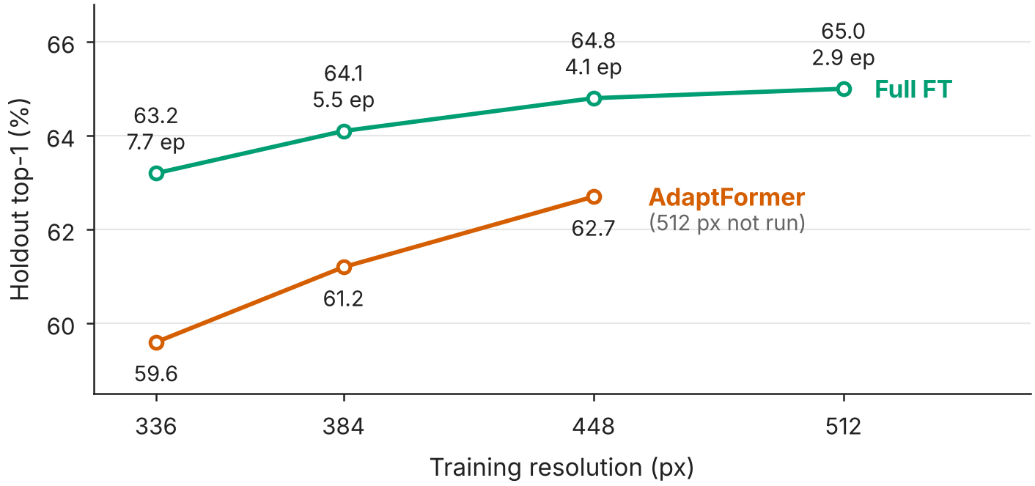
\includegraphics[width=0.68\textwidth]{media/media/image3.png}}{Resolution at equal compute. Full fine-tuning flattens after 448 px; AdaptFormer keeps improving to 448 px.}{fig:resolution}


\subsection{PEFT comparisons}\label{peft-comparisons}

\textbf{Method comparison (RQ2).} At 336 px and the same 144-minute budget, six methods perform within a narrow range (77.6--78.5\%). We treat these as ties, because recipes and batch sizes differ between methods (Table~\ref{tab:peft}). Methods with much smaller budgets, or that adapt only one block, fall clearly behind. Which parameters are trained matters more than how many: BitFit trains only 0.12\% of the backbone and reaches 73.4\%, whereas last-block attention trains 2.75\% and reaches only 67.9\%. In general, methods that add capacity to every block outperform those that concentrate it in one place. AdaLoRA scored 2.7 pp below LoRA on the 1,000-class pilot, so it was not run at full scale.



\staytable{%
\scriptsize
\begin{tabularx}{\textwidth}{@{}Xcccc@{}}
\toprule
Method & Backbone trained & Top-1 (\%) & VRAM (GiB) & Latency (ms) \\
\midrule
Last-block attention & 2.75\% & 67.93 & 1.43 & 7.76 \\
Prefix, length 50 & 1.07\% & 72.1 & 7.97 & 9.64 \\
BitFit, all biases & 0.12\% & 73.4 & 7.01 & 7.40 \\
Serial adapter w96 + extras & 4.68\% & 77.6 & 15.54 & 11.60 \\
GPS & 4.63\% & 77.9 & 20.37 & 7.13 \\
AdaptFormer w192 & 4.13\% & 77.9 & 14.53 & 10.28 \\
DoRA r24 + extras & 4.75\% & 78.3 & 28.06 & 23--24 (7.71) \\
LoRA r24 & 4.12\% & 78.4 & 19.30 & 15.37 (7.78) \\
LoRA r24 + extras & 4.65\% & 78.5 & 19.40 & 14.2--15.0 (7.68--8.35) \\
\bottomrule
\end{tabularx}}{PEFT methods on validation at 336 px with no prediction-time extensions and a 144-minute budget. Small differences should be read as ties because recipes and physical batches differ. Parentheses show latency after merging.}{tab:peft}


\textbf{Cost.} The share of trainable parameters predicts neither memory use nor latency. BitFit trains only 0.12\% of the backbone but still needs 7.0 GiB, because gradients must flow back through every block. Last-block attention stops backpropagation at block 12 and needs only 1.43 GiB. At inference, adapters, AdaptFormer and prefixes remain in the forward pass and add latency, whereas LoRA and DoRA add none once merged into the weights.

\textbf{Where the parameters go.} Training the biases and LayerNorm weights in every block improved AdaptFormer by 0.50 pp (76.26\% $\rightarrow$ 76.76\%) at a cost of only 0.14\% of the backbone. At an equal budget, spreading parameters across all 12 blocks or only the last 8 made no difference, for both LoRA (77.26\% vs. 77.33\%) and AdaptFormer (76.77\% vs. 76.90\%), averaged over two seeds.

\textbf{What kind of capacity.} Starting from AdaptFormer at 4.26\% of the backbone (76.77\%), widening the adapters to 4.94\% gave no gain (76.84\%), whereas spending the same extra budget on LoRA improved accuracy by 0.6 pp in both seeds (77.43\%). LoRA alone at the same budget performed on par with AdaptFormer + LoRA (77.26\%).

\textbf{Building the final PEFT design.} On the holdout (336 px, 3 epochs), AdaptFormer with the default recipe reached 75.27\%. The cosine margin and related changes added 0.99 pp, bias and LayerNorm tuning 0.50 pp and LoRA 0.66 pp, giving 77.43\% at 4.94\% of the backbone. On the validation set, the design went from 77.9\% (336 px) to 79.4\% (+ biases and LayerNorms, 384 px), 80.4\% (448 px), 81.2\% (+ LoRA), 82.2\% (+ zoom) and 83.08\% (+ kNN); since some steps change two factors at once, this traces how the design was built rather than isolating each step.

\subsection{Overfitting: Validation vs. Test Set}\label{overfitting-validation-vs.-test-set}

Every design choice was guided by validation accuracy, so we check for overfitting by scoring the best model on the 100,000 unseen test images (Table~\ref{tab:test}). Accuracy drops by only 0.2--0.3 pp, and the kNN gain holds (+0.93 vs. +0.85 pp) because its settings were fixed on the labelled holdout rather than on the validation set. The model therefore shows little sign of overfitting to the validation set.



\staytable{%
\small
\begin{tabularx}{\textwidth}{@{}Xccc@{}}
\toprule
 & Validation & Test & Change \\
\midrule
Zoom & 83.22 & 82.91 & $-0.31$ \\
Zoom + kNN & 84.07 & 83.84 & $-0.23$ \\
kNN gain & +0.85 & +0.93 & -- \\
\bottomrule
\end{tabularx}}{Validation versus test accuracy for full fine-tuning at 448 px.}{tab:test}


\textbf{Fitting vs. generalisation.} AdaptFormer fits its training images almost as well as full fine-tuning (95.0\% vs. 95.5\% top-1) but scores 1.4 pp lower on the holdout (77.45\% vs. 78.81\%; Appendix, Table~\ref{tab:train-holdout}). The PEFT gap therefore comes from how well the learned features generalise, not from too little capacity to fit the data, which is consistent with wider adapters giving no gain (Section 5.3). Holdout accuracy still rises through epoch 3 for both models. Full fine-tuning starts 3.7 pp behind, draws level at epoch 2 and leads at epoch 3, so its advantage comes late rather than from a faster start.

\subsection{Error analysis}\label{error-analysis}

To understand what limits the adapted model (RQ3), we analysed the 11,111 errors made by LoRA (rank 24, 336 px) on the 10,000-class labelled holdout (top-1 accuracy 77.8\%). For each error, we asked where the true class was ranked.

\textbf{Most errors are near misses.} Top-1 accuracy is 77.8\%, but top-2 accuracy is 86.0\%, top-5 is 92.0\% (Appendix, Figure~\ref{fig:topk}). Among the errors, the true class is ranked second in 37\% of cases, third to fifth in 27\%, and outside the top five in 36\%. Most errors are therefore near misses: the correct class is on the model's shortlist but ranked too low. Re-ordering the shortlist could correct these errors without retraining, which motivates kNN re-ranking (Section 3.6). Errors outside the top five, by contrast, would require a better model rather than better ranking.

\subsection{Prediction-time extensions}\label{prediction-time-extensions}

Zoom and kNN re-ranking each improve accuracy without retraining, and their gains are nearly additive. For LoRA (rank 24, 336 px, centre crop 0.75) on the holdout, zoom adds 0.7 pp, kNN adds 1.3 pp and both together add 2.0 pp (78.31\% $\rightarrow$ 80.27\%; Appendix, Figure~\ref{fig:zoom-knn}). An equal-cost ablation shows that most of zoom's gain comes from seeing the object at higher resolution rather than from averaging two passes (Appendix, Table~\ref{tab:second-view}; examples in Figure~\ref{fig:zoom-examples}).

An ablation over six kNN scoring rules (Appendix, Table~\ref{tab:knn}) shows that scoring against individual training images beats scoring against a class summary: the mean similarity to the 3 closest images adds 1.32 pp, the class-mean feature 0.55 pp, and the mean over all of a class's images only 0.13 pp. A class can look quite different across its images, and an image showing a less common appearance may closely match a few training images but not the class average. On the holdout (LoRA rank 24, no zoom), kNN corrected 12\% of the holdout errors (1,376 of 11,111), and it can only reach the 64\% of errors whose true class is in the top five. Most fixes (1,089) were errors where the true class was ranked second: kNN corrected about a quarter of those but only about one in ten when the true class was ranked third to fifth, likely because the similarity bonus can overturn a small score gap but rarely a larger one.

\textbf{Cost.} Once the feature bank exists, kNN adds less than 0.1 ms per image. However, the 0.7 GB bank takes 25--30 minutes to build at 448 px and must be rebuilt whenever the model changes. Zoom costs about 2.7--2.8$\times$ a single pass at batch size 1 (23.43 vs. 8.47 ms for full fine-tuning).

\section{Discussion and conclusion}\label{discussion-and-conclusion}

\textbf{RQ1: Full fine-tuning vs. PEFT.} A well-tuned fully fine-tuned model outperforms the best PEFT model by about 1.0 pp on the validation set (84.07\% vs. 83.08\%) and reaches 83.84\% on the unseen test set. It is also faster at inference, but only because our PEFT model uses AdaptFormer, whose branch cannot be merged; a merged LoRA adds no latency (Table~\ref{tab:peft}). PEFT trains only 4.94\% of the backbone and uses less memory, but saves no training time: both methods completed 5.5 epochs in the same 144 minutes. PEFT is often preferred on small datasets, but although we have only 45 images per class, the 10,000 classes give 450,000 training images, which may explain why full fine-tuning wins here.

\textbf{RQ2: spending a PEFT budget.} Which parameters are trained matters more than how many. Tuning biases and LayerNorm weights in every block is cheap and worth including. Once every block can adapt, the placement of additional parameters has little effect, and LoRA is a more efficient way to add capacity than widening the adapters. The classification head and learning-rate settings had a larger effect than the choice among the strongest PEFT methods, which performed within 1 pp of each other.

\textbf{RQ3: What limits the adapted model.} Most remaining errors are near misses: the true class is in the top five for 64\% of errors and ranked second for 37\%. Modifying the loss to separate related classes did not help in our pilots (for example, label smoothing towards neighbouring classes gave 63.92\% vs. 64.06\% at 384 px, a tie). What did help was giving the model more information: higher input resolution during training, a zoomed second view, and comparison with individual training images. The last two require no training, and the kNN gain held on the unseen test set (+0.93 pp vs. +0.85 pp on validation).

\textbf{Limitations and future work.} Our conclusions come from one backbone (ViT-B/16), one dataset and one compute budget (144 minutes per run; Section 3.1), so the size of the full-FT advantage may change with a larger model, more data per class or a longer budget. Because only two test submissions were allowed, PEFT was compared with full fine-tuning on the validation set, which also guided our design choices; scoring both final systems on held-out test data would make the comparison firmer. Our PEFT design keeps AdaptFormer for faster training, at the cost of slower inference, but LoRA alone matched its accuracy. A LoRA-only design, merged after training, could therefore remove the latency penalty and is the natural next step for latency-sensitive deployment. Finally, the prediction-time extensions are not free: zoom needs a second forward pass, and kNN needs a 0.7 GB feature bank that must be rebuilt for each new model. Learning the zoom or the neighbour comparison during training could keep their gains without this cost.

\textbf{Conclusion.} The better adaptation depends on the deployment's priority. For accuracy, full fine-tuning wins by about 1 pp (84.07\% vs 83.08\%). For memory and storage, PEFT wins: 4.94\% of the backbone trained, 3.1 GiB less training memory, and 48 MB per task instead of 375 MB. For latency, use full fine-tuning or a mergeable method such as LoRA. Training time does not separate them. At prediction, zoom suits tasks where the deciding detail is small, and kNN suits tasks whose errors are mostly near misses between classes with varied appearances. Because these choices interact, resolution, optimisation, parameter placement and prediction should be tuned together.

\bibliographystyle{iclr2026_conference}
\bibliography{refs}

\clearpage
\appendix
\setcounter{figure}{0}
\renewcommand{\thefigure}{A\arabic{figure}}
\renewcommand{\theHfigure}{A\arabic{figure}}
\setcounter{table}{0}
\renewcommand{\thetable}{A\arabic{table}}
\renewcommand{\theHtable}{A\arabic{table}}
\section{Appendix}\label{appendix}

\stayfig{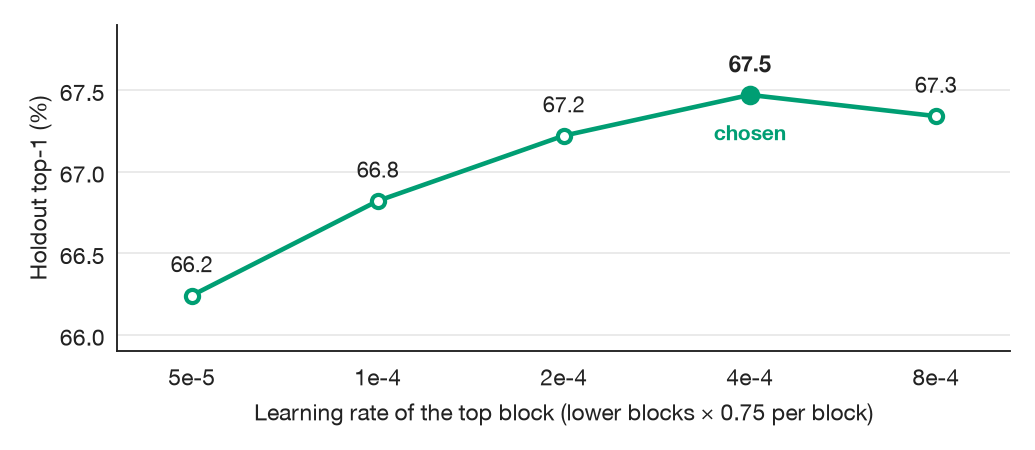
\includegraphics[width=0.82\textwidth]{media/media/image4.png}}{Learning-rate sweep for full fine-tuning with layer-wise decay 0.75.}{fig:lr-sweep}

\stayfig{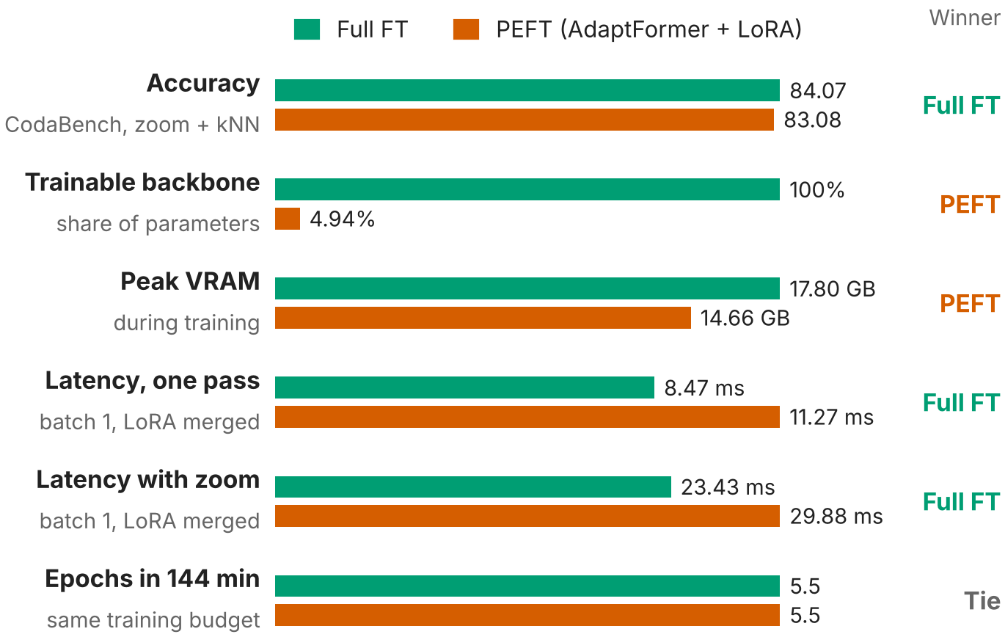
\includegraphics[width=0.82\textwidth]{media/media/image5.png}}{Full fine-tuning versus AdaptFormer + LoRA across accuracy, memory, parameters, time and latency.}{fig:summary}

\stayfig{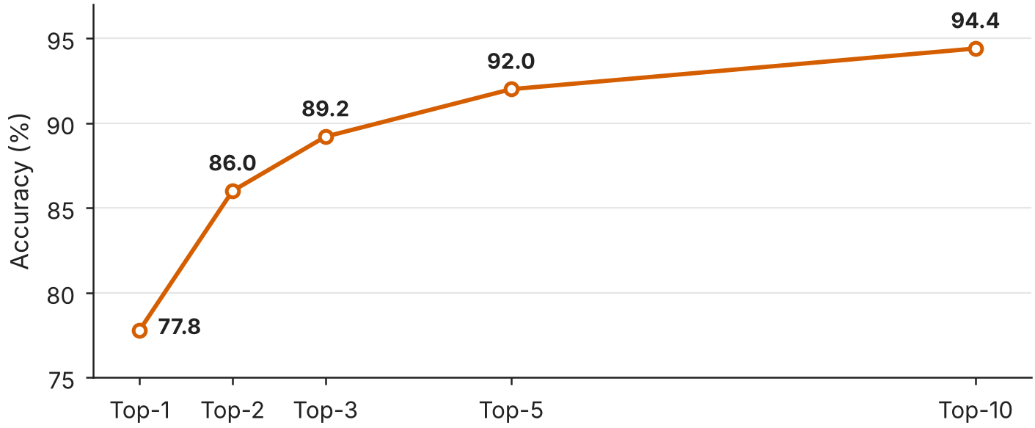
\includegraphics[width=0.82\textwidth]{media/media/image6.png}}{Top-k holdout accuracy: the correct class is usually on the short list.}{fig:topk}

\stayfig{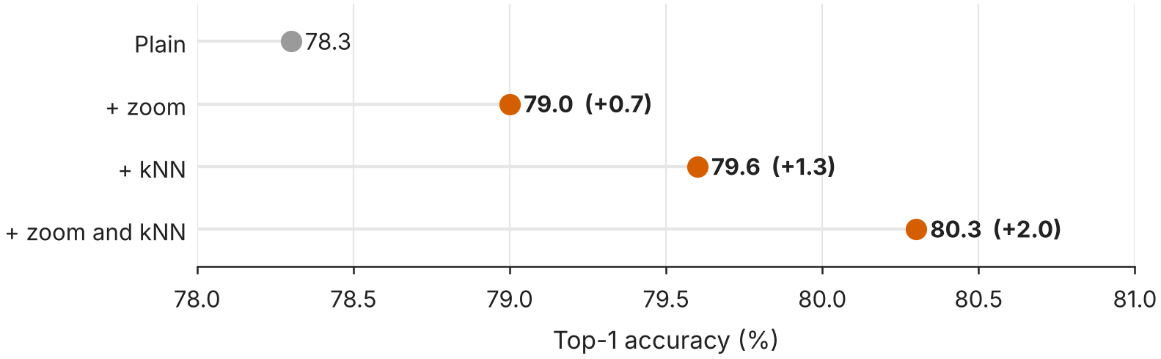
\includegraphics[width=0.82\textwidth]{media/media/image7.png}}{Zoom and kNN gains on the all-class holdout.}{fig:zoom-knn}

\stayfig{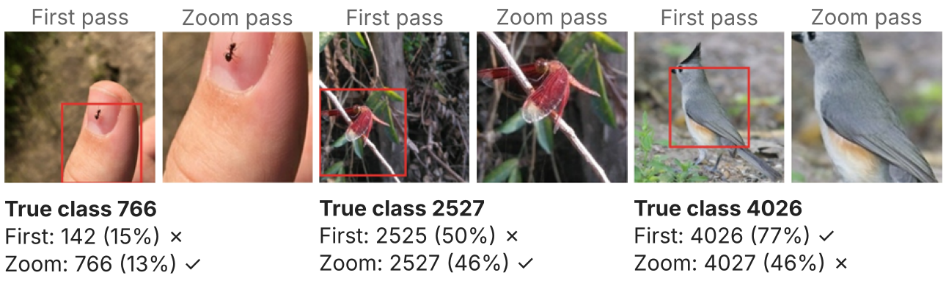
\includegraphics[width=0.82\textwidth]{media/media/image8.png}}{Examples where attention-guided zoom changed the prediction.}{fig:zoom-examples}

\staytable{%
\small
\begin{tabularx}{\textwidth}{@{}Xccc@{}}
\toprule
 & Epoch 1 & Epoch 2 & Epoch 3 \\
\midrule
AdaptFormer, training & 82.91 & 92.48 & 94.97 \\
AdaptFormer, holdout & 70.26 & 76.06 & 77.45 \\
AdaptFormer, gap & 12.66 & 16.41 & 17.52 \\
Full FT, training & 78.17 & 91.78 & 95.46 \\
Full FT, holdout & 66.55 & 76.00 & 78.81 \\
Full FT, gap & 11.62 & 15.78 & 16.65 \\
\bottomrule
\end{tabularx}}{Training and holdout accuracy per epoch.}{tab:train-holdout}

\staytable{%
\small
\begin{tabularx}{\textwidth}{@{}Xr@{}}
\toprule
Second view & Gain (pp) \\
\midrule
Horizontal flip & +0.17 \\
Centre crop & +0.63 \\
Activation-guided zoom & +0.79 \\
\bottomrule
\end{tabularx}}{Equal-cost second views for full fine-tuning (336 px holdout; baseline 78.80\%).}{tab:second-view}

\staytable{%
\small
\begin{tabularx}{\textwidth}{@{}lXcc@{}}
\toprule
Variant & Query comparison & Gain (pp) & On top of zoom \\
\midrule
kNN, mean of 3 & Mean cosine to three closest class images & +1.32 & +1.23 \\
kNN, best match & Cosine to closest image & +1.18 & +1.02 \\
Weighted vote & 50 nearest images of any class & +1.14 & +1.03 \\
3 k-means centres & Best cosine to three class centres & +0.70 & +0.69 \\
Class mean & Cosine to average class feature & +0.55 & +0.49 \\
kNN, mean of all & Mean cosine to all class images & +0.13 & +0.13 \\
\bottomrule
\end{tabularx}}{kNN scoring variants on the holdout.}{tab:knn}

\end{document}
